\section{ArtBot's Workflow (Fabio Aubele)}\label{sec:flow}
Der grundlegende Arbeitsablauf des entwickelten Chatbot ist bereits von Rasa vorgegeben. Grafik \ref{flow} beschreibt diesen genauer.
\begin{figure}[htbp]
	\centerline{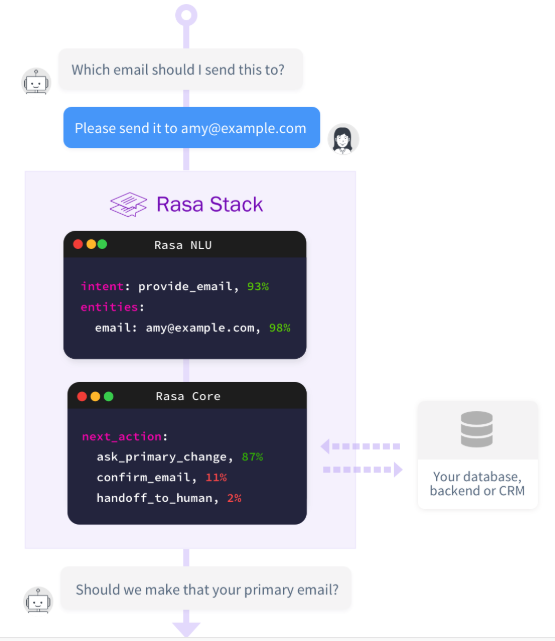
\includegraphics[width=1\linewidth]{figures/rasa_full.jpg}}
	\caption{Genereller Workflow von ArtBot.}
	\label{flow}
\end{figure}
Zunächst ist nur die Äußerung des Benutzers vorhanden. Diese wird dann von Rasa NLU verarbeitet, als Ergebnis werden Intent und Entities ausgegeben. Daraufhin werden diese von Rasa Core benutzt, um die nächste auszuführende Aktion des Chatbots zu ermitteln. Dies können normale textuelle Äußerungen sein, welche einfach wiedergegeben werden oder es wird externer Python-Code aufgerufen. Innerhalb der entwickelten Anwendung führt dieser Code immer Datenbankabfragen aus, womit überprüft wird, ob der von dem Benutzer genannte Maler oder das genannte Kunstwerk in der Datenbank vorhanden ist. Falls dies zutrifft, wird das gewünschte Kunstwerk angezeigt. Hierbei gibt es unterschiedliche Möglichkeiten für den Benutzer, nach einem Bild zu fragen. Diese sind dabei in Kapitel \ref{sec:dialog} aufgezeigt. Die nächsten beiden Kapitel erklären die Arbeitsabläufe in Rasa NLU und Rasa Core genauer. Um den grundlegenden Aufbau und alle Begrifflichkeiten rund um Rasa zu verstehen, empfiehlt es sich, davor die dazugehörige Seminar-Arbeit (Quelle \cite[S.9-11]{seminar}) durchzulesen.

\subsection{Rasa NLU}\label{sec:flownlu}
Rasa NLU transformiert die Äußerung des Benutzers in einen jeweiligen Intent und endlich vielen Entities. Um diesen Schritt zu ermöglichen, müssen erstmals alle nötigen Intents und Entities angegeben werden. Dies geschieht durch eine Markdown- oder Json-Datei in der von Rasa vorgegebenen Formatierung.\\
Um die Umwandlung zu vollziehen, benötigt es die sogenannte Pipeline von Rasa. Diese setzen sich aus mehreren Komponenten zusammen, welche allesamt zusammenarbeiten. Der Kernbestandteil ist ein Machine Learning Algorithmus, welcher die gewünschten Entities erkennt und ein neuronales Netz, welches die Sätze mit dem jeweils korrekten Intent klassifiziert. Rasa bietet dabei vorkonfigurierte Pipelines an, die für häufig vorkommende Use-Cases optimiert sind. Eine Übersicht der einzelnen Bestandteile und der vorkonfigurierte Pipelines bietet Quelle \cite{nlunn} an.\\
\\
Innerhalb dieser Arbeit wurde die vorkonfigurierte Pipeline 'supervised\_embeddings' verwendet. Diese ermöglicht es, Anwendungen in anderen Sprachen (der Standard ist Englisch) zu formulieren und da der entwickelte Chatbot nur auf deutsche Angaben reagieren soll, eignet sich diese Pipeline optimal. Die einzelnen Bestandteile sind in Abbildung \ref{se} aufgelistet.
\begin{figure}[htbp]
	\centerline{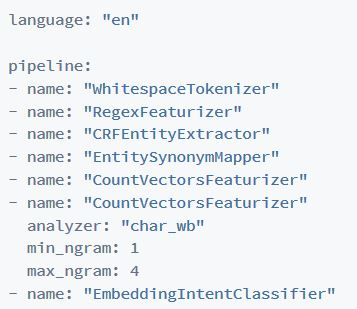
\includegraphics[width=0.5\linewidth]{figures/se.jpg}}
	\caption{Bestandteile der 'supervised\_embeddings' Pipeline \cite{nlunn}.}
	\label{se}
\end{figure}
Die angegebene Sprache in der ersten Zeile wurde für ArtBot in 'de' für deutsch abgeändert. Der nun erste Teil der Pipeline ist der 'WhitespaceTokenizer', welcher die einzelnen Wörter der Äußerung des Nutzers anhand von Leerzeichen trennt. Darauf folgt der 'RegexFeaturizer', der benötigt wird, um reguläre Ausdrücke zu erkennen. Dies wird in dieser Anwendung jedoch nicht benutzt. Nun folgt der 'CRFEntityExtractor', welcher einer der wichtigsten Bestandteil der Pipeline ist, da sich dieser um die Extraktion der Entities kümmert. Hierbei wird ein Conditional Random Field (CRF) Model aus der Python-Bibliothek 'scikit-learn'\footnote{siehe \href{https://scikit-learn.org/stable/}{https://scikit-learn.org/stable/}} verwendet \cite{nlunn}. Ein CRF-Model ist ein 'Discriminative Model', welches zum Erkennen von Pattern eingesetzt wird und somit häufig benutzt wird, um Vorhersagen in sequenziellen Daten zu treffen \cite{crf}. Dabei werden kontextuelle Informationen benötigt. Dies ist auch der Grund, dass sich dieser Algorithmus sehr gut eignet, um Entities zu erkennen, da diese stark von den vorherigen und nachfolgenden Wörtern abhängen. Eine detaillierte Erklärung des CRF-Model bietet Quelle \cite{crf} an.\\
Der nächste Bestandteil ist der 'EntitySynonymMapper', mit dessen Hilfe den Entities Synonyme zugeordnet werden können. Dies wird allerdings in der entwickelten Anwendung ebenfalls nicht verwendet. Dann folgen zwei 'CountVectorsFeaturizer', welche Merkmale aus den gegebenen Wörtern ableiten, die von dem 'WhitespaceTokenizer' extrahiert worden sind. Anhand dieser Merkmale kann der nächste Teil der Pipeline die vorliegende Klassifizierungsaufgabe lösen. Der erste 'CountVectorsFeaturizer' benötigt dafür nur die extrahierten Wörter. Die zweite Instanz benutzt N-Gramme, welche die einzelne Buchstaben der Wörter neu zusammenfügt und dann die Erzeugnisse zum Erstellen von Merkmalen anwendet. Die darunter stehenden Argumente sind die Einstellungen, welche zur Erzeugung der N-Gramme verwendet werden. Diese geben die minimale (1) und maximale Länge (4) an, sowie die eingesetzte Methode (char\_wb), welche angibt, dass nur Zeichen innerhalb der definierten Grenze hergenommen werden dürfen. Für eine genauere Erklärung von N-Grammen siehe Referenz \cite{ngramm}.\\
\\
Zu guter Letzt folgt der 'EmbeddingIntentClassifier', welcher der wichtigste Teil der Pipeline ist, da dieser die Klassifizierungsaufgabe löst und den finalen Intent ausgibt. Dieser benutzt ein neuronales Modell namens StarSpace, welches in Quelle \cite{starspace} detailliert vorgestellt wird. Dabei werden die durch den 'CountVectorsFeaturizer' erstellten Merkmale benötigt, um dem gegebenen Satz den korrekten Intent zuzuordnen. Der Aufbau des neuronalen Netzes ist in Abbildung \ref{star} zu sehen.
\begin{figure}[htbp]
	\centerline{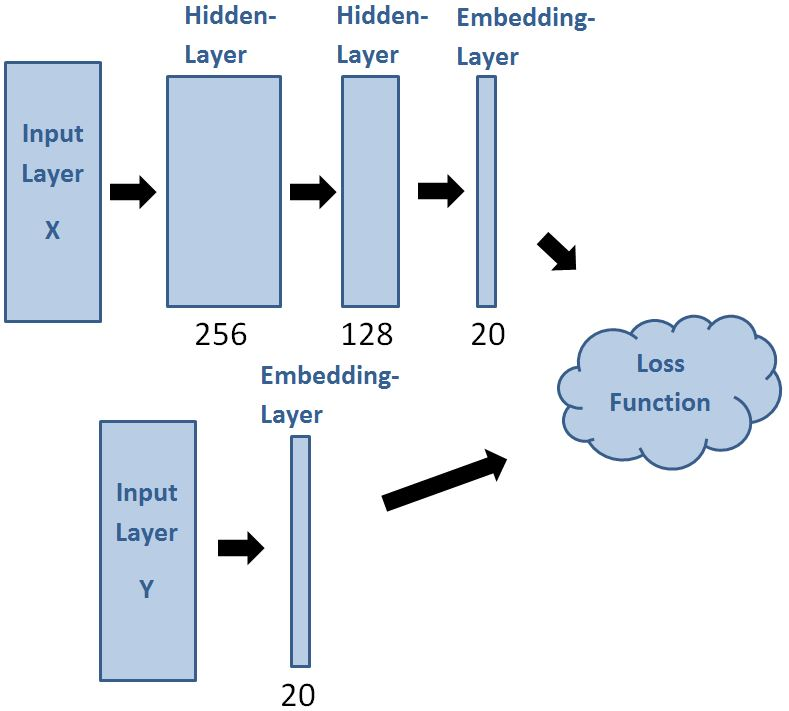
\includegraphics[width=0.8\linewidth]{figures/star.jpg}}
	\caption{Aufbau des neuronalen Netzes zur Intent-Erkennung (basierend auf \cite{ftech}).}
	\label{star}
\end{figure}
Dabei gibt es zwei getrennte Netze, eines für die Eingabe des Benutzers (X) und eines für die definierten Intents (Y), welche als Label verwendet werden. Die Eingaben des Benutzers werden durch zwei Hidden-Layers geführt, mit 256 Neuronen und 128 \cite{ftech}. Daraufhin folgt der Embedding Layer (20 Neuronen), welche die Buchstaben in einen Zahlenvektor umwandelt. Die Intents werden nur durch den Embedding Layer geführt \cite{ftech}. Zuletzt wird mittels einer Loss-Function die Unähnlichkeit der Ergebnisse beider Embedding Layers bestimmt. Dafür wird die Kosinus-Ähnlichkeit benutzt \cite{ftech}. Der am wenigsten unähnliche Intent wird als Klassifizierungsergebnis bestimmt.\\
\\
Mithilfe dieses Vorgehens lässt sich das neuronale Netz trainieren, um die optimalen Gewichte zwischen den einzelnen Layern zu finden. Daraufhin kann das Netz später eingesetzt werden, um den Äußerungen des Nutzers einen Intent zuzuordnen. Die Intents müssen dabei vorher bereits definiert worden sein, um das Netz für diese zu trainieren. Rasa ermöglicht dem Entwickler bestimmte Einstellungen des Netzes zu ändern und anzupassen, innerhalb von ArtBot werden jedoch die Standard Einstellungen benutzt. Eine Übersicht der Standardeinstellungen und aller änderbaren Eigenschaften sind in Quelle \cite{embedd} aufgelistet.\\
Final erhält die Anwendung durch diese Pipeline und somit durch Rasa NLU den Intent und die verwendeten Entities innerhalb einer Äußerung des Benutzers.

\subsection{Rasa Core}\label{sec:flowcore}
Rasa Core verwendet den gegebenen Intent und die gegebenen Entities, um die nächste Aktion des Chatbots zu ermitteln. Dabei wird unterschieden zwischen 'utterance-actions', was normale textuelle Äußerungen des Chatbots sind und 'custom-actions', welche externe Logik mit Hilfe von Python-Code ausführen. Für die entwickelte Anwendung ArtBot werden 'custom-actions' nur benötigt, um Eingaben zu überprüfen sowie aus der anhängenden Datenbank Informationen zu holen und diese auszugeben.\\
Um diese Funktionalität zu ermöglichen, müssen vorerst sogenannte Stories angelegt werden. Diese widerspiegeln den Gesprächsfluss des Benutzers und des Chatbots. Definiert werden diese in einer von Rasa vorgegebenen Form innerhalb von Markdown-Dateien. Zusätzlich fungieren diese Stories als Trainingsdaten für die Policies.\\
\\
Rasa Core verwendet Policies, um die nächste auszuführende Aktion des Chatbots algorithmisch zu ermitteln. Nun gibt es mehrere vorkonfigurierte Policies für verschiedene Anwendungsfälle. In der entwickelten Anwendung ArtBot wurden folgende benutzt:
\begin{itemize}
	\setlength\itemsep{-0.6em}
	\item MemoizationPolicy
	\item MappingPolicy
	\item KerasPolicy
\end{itemize}
Die MemoizationPolicy sagt die nächste Aktion mit einer Wahrscheinlichkeit von 1.0 vorher, wenn die Konversation mit dem aktuellen Nutzer mit einer Konversation aus den Trainingsdaten übereinstimmt. Hierbei merkt sich die Policy die Konversationen aus den Trainingsdaten und vergleicht diese dann. Gibt es keine Übereinstimmungen wird None (Datentyp in Python) vorhergesagt mit einer Wahrscheinlichkeit von 0.0. Tritt dieser Fall ein, wird sich auf das Ergebnis der anderen Policies verlassen.\\
Etwas anders funktioniert die MappingPolicy, welche die Trainingsdaten nicht benötigt. Hier muss bei der Definition eines Intents innerhalb der Domain das Attribut 'triggers' verwendet werden, ansonsten wird diese Policy nicht ausgelöst. Ein Beispiel dafür ist in Code \ref{trigger} zu sehen.
\begin{lstlisting}[caption={Verwendung der MappingPolicy innerhalb von ArtBot.}, label=trigger, lineskip=1pt, morekeywords={intents, greet, goodbye}]
intents:
  - greet:
    triggers: action_greet
  - goodbye:
    triggers: utter_goodbye
...
\end{lstlisting}
Durch dieses Konstrukt löst der Intent \texttt{greet} nun immer \texttt{action\_greet} aus, was eine 'custom-action' ist und der Intent \texttt{goodbye} immer \texttt{utter\_goodbye}, was wiederum eine 'utterance-action' ist.\\
\\
In den meisten Fällen wird jedoch die KerasPolicy angewendet, welche die gleichnamige Python-Bibliothek Keras\footnote{siehe \href{https://keras.io/}{https://keras.io/}} benutzt. Dafür wird ein neuronales Netz mit der Long Short Term Memory (LSTM) Architektur verwendet, welches ein Recurrent Neural Network (RNN) ist. LSTM's haben die Möglichkeit langfristige Abhängigkeiten festzuhalten. Dabei werden sich Informationen gemerkt und für spätere Zusammenhänge wiederverwendet. Diese Eigenschaft ist für Chatbots besonders wichtig, da der Gesprächsverlauf auch durch frühe Dialogentscheidungen beeinflussbar sein muss. Eine detaillierte Erklärung der LSTM Architektur und seiner Eigenschaften bietet Quelle \cite{lstm}. In Rasa soll der Dialog durch folgende drei Faktoren zusätzlich beeinflussbar sein \cite{rasa}:
\begin{itemize}
	\setlength\itemsep{-0.6em}
	\item Was war die letzte Aktion des Chatbots?
	\item Was ist der Intent und die Entities der letzten Nachricht des Benutzers?
	\item Welche Slots sind momentan belegt?
\end{itemize} 
Um dies zu realisieren benötigt es die in Abbildung \ref{lstm} vereinfacht beschriebene Architektur.
\begin{figure}[htbp]
	\centerline{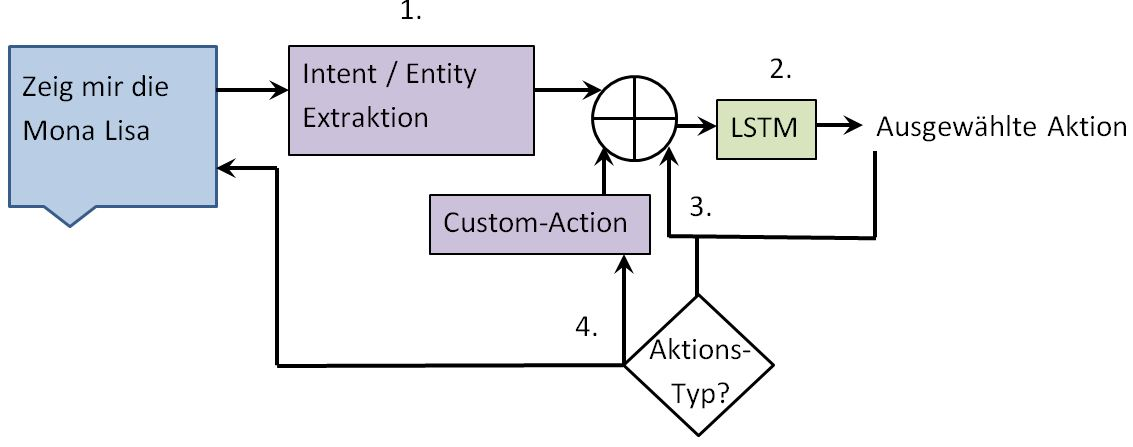
\includegraphics[width=1\linewidth]{figures/lstm.jpg}}
	\caption{Aufbau von LSTM in Rasa Core (basierend auf \cite{lstmrasa}).}
	\label{lstm}
\end{figure}
\\Zunächst werden in Schritt eins Intent und Entity durch Rasa NLU extrahiert. Daraufhin folgt der Aufruf von LSTM in Schritt zwei. Hier nimmt LSTM nicht nur Rücksicht auf den momentanen Intent und die momentanen Entities, sondern auch auf die vorherigen aufgerufenen Aktionen, welche sich für weitere Vorhersagen gemerkt werden (dargestellt durch den Kreis) \cite{lstmrasa}. LSTM wählt anhand dieser Informationen und den als Trainingsdaten verwendeten Stories nun die nächste Aktion aus. Daraufhin wird diese in Schritt 3 wieder als Information für den nächsten Aufruf hinterlegt (Kreis) \cite{lstmrasa}, damit LSTM weiterhin die zuletzt ausgeführte Aktion kennt. Dann wird in Schritt 4 entschieden, was für ein Typ die von LSTM ausgewählte Aktion ist \cite{lstmrasa}. Bei einer 'custom-action' wird der entsprechende Python-Code aufgerufen und ausgeführt. Hier kann es sein, dass die 'custom-action' zusätzliche Aktionen ausführt oder Slots abändert. Dies wird daraufhin wieder als Information hinterlegt (Kreis). Ist die Aktion jedoch eine 'utterance-action' wird der Text nur ausgegeben. Es kann auch passieren, dass die ausgewählte Aktion in Schritt 2 lediglich einen Slot abändert. Dies wird ebenfalls für den nächsten Aufruf hinterlegt (Kreis), jedoch folgt keine Ausgabe von Text oder die Ausführung einer 'custom-action'.\\
Für eine noch detaillierte Erklärung der Verwendung von LSTM innerhalb von Rasa steht Quelle \cite{lstmrasa} zur Verfügung. Wie genau LSTM aufgebaut ist und wie groß das dadurch aufgespannte Netz ist, wurde von Rasa nicht dokumentiert.\\
Rasa Core ermöglicht somit, die korrekte Aktion des Chatbots für eine Äußerung des Nutzers zu ermitteln und diese auszuführen, wie in den Stories vermerkt. Zusammen mit Rasa NLU und der implementierten Datenbank-API wird somit der in Abbildung \ref{flow} dargestellte Workflow realisiert.

\subsection{Gesprächsfälle}\label{sec:dialog}
Bei der Erstellung der Trainingsdaten, mit welchen die in den Kapiteln \ref{sec:flownlu} und \ref{sec:flowcore} beschriebenen Netze trainiert werden, wurde darauf geachtet, dass es dem Chatbot möglich ist, auf mehrere unterschiedliche Gesprächsfälle einzugehen. Diese sollen in diesem Abschnitt erläutert werden. Auch wurde ein Teil der Logik innerhalb der 'custom-actions' implementiert. Hier wird geprüft, ob die Angaben zu Künstler und Kunstwerk korrekt sind und in der Datenbank auch vorkommen. Wie bereits erwähnt, ist der generelle Anwendungsfall Bilder anzuzeigen, nachdem der Künstler und das Kunstwerk von dem Benutzer genannt wurde.\\
\\
Grundlegend kann für den Künstler immer der volle Name oder nur der Vorname bzw. der Nachname angegeben werden. Gibt es dabei mehrere Künstler, welche zum Beispiel den selben Vornamen haben, werden alle in Frage kommende Künstler aufgelistet (z.B. bei Paul: Paul Gauguin, Paul Cezanne und Peter Paul Rubens), damit der Benutzer einen davon in der nächsten Eingabe auswählen kann. Das gleiche gilt auch für Kunstwerke. Hier kann der volle Titelname genannt werden, welcher in dem benutzten Datensatz immer einzigartig ist oder nur der Anfang eines Titels (z.B. 'Resurrection' für 'Resurrection of Lazarus'). Gibt es mehrere Bilder mit dem selben Anfang, werden alle aufgelistet (z.B. Portrait: 'Portrait of a Young Man' oder 'Portrait of Gaspard Schoppins'), damit der Benutzer wieder eines auswählen kann. Falls der Benutzer nicht den exakt korrekten Titel des Kunstwerkes oder Namen des Künstlers nannte, gibt der Chatbot innerhalb einer Extra-Ausgabe den jeweils korrekten Wert an.\\
\\
Nun gibt es drei mögliche Fälle, auf welcher Art der Benutzer nach einem Kunstwerk fragen kann: 
\begin{enumerate}
	\setlength\itemsep{-0.6em}
	\item Der Benutzer nennt Künstler und Kunstwerk in einer Äußerung.
	\item Der Benutzer nennt erst den Künstler in einer Äußerung und daraufhin das Kunstwerk.
	\item Der Benutzer nennt nur das Kunstwerk in einer Äußerung.
\end{enumerate}
Für den ersten Fall müssen sowohl der Künstler, als auch das Kunstwerk in der Datenbank vorhanden sein. Ansonsten wird angegeben, welcher Wert falsch war. Sind beide Werte korrekt wird das Bild angezeigt.\\
Innerhalb des zweiten Falles nennt der Nutzer zuerst den Künstler, welcher wiederum in der Datenbank stehen muss oder es wird angegeben, dass der Künstler nicht vorhanden ist. Daraufhin wird dem Benutzer eine Auswahl der zur Verfügung stehende Kunstwerke dieses Künstlers aufgelistet. Hier kann der Benutzer nun eines dieser Werke auswählen, wenn der Benutzer das Kunstwerk korrekt wiedergibt und es somit in der Datenbank vorhanden ist, wird es daraufhin angezeigt. Nach dem Benennen eines Künstlers muss der Benutzer kein Kunstwerk angeben, er kann auch je nach Belieben wieder einen der drei oben genannten Fälle auslösen.\\
Für den letzten Fall kann der Benutzer nur den Titel eines Kunstwerkes nennen, welches sofort angezeigt wird, wenn es in der Datenbank vorhanden ist. Ansonsten gibt ArtBot an, dass ein solches Kunstwerk nicht existiert. Hier kann auch der Fall auftreten, dass der Titel zu ungenau ist, dabei werden, wie oben erwähnt, alle in Frage kommende Bilder aufgelistet.\\
\\
Diese Modellierung der Gesprächsfälle erlaubt es auch, nur einen Intent anlegen zu müssen, was die Implementation erleichtert. Eine Fallunterscheidung kann gemacht werden, indem geprüft wird, wie viele Entities der Nutzer angegeben hat. Dies wird von Rasa unterstützt, wodurch kein zusätzlicher Programmieraufwand entsteht. Insbesondere bei ähnlichen Äußerungen schlägt Rasa ein solches Vorgehen sogar vor. Dies bedeutet für Fall 1 werden beide Entities (Künstler und Titel des Kunstwerkes) benötigt, für Fall 2 nur der Künstler und bei Fall 3 nur der Titel des Kunstwerkes.
